\documentclass[a4paper,10pt]{report}

%%%% PRATIQUE POUR LES ALINEAS CHIANTS
\usepackage{indentfirst}

\usepackage[colorlinks=false]{hyperref}

%%%% POUR L'OPTION LABEL= %%%
\usepackage{enumitem}

\setlength{\parindent}{30pt}
\setlength{\parskip}{1ex}
\setlength{\textwidth}{15cm}
\setlength{\textheight}{24cm}
\setlength{\oddsidemargin}{0.2cm}
\setlength{\evensidemargin}{-.7cm}
\setlength{\topmargin}{-.5in}

\usepackage{graphicx}
\usepackage{titling}
\usepackage{listings}
\lstset{%
  basicstyle=\scriptsize\sffamily,%
  commentstyle=\footnotesize\ttfamily,%
  frameround=trBL,
  frame=single,
  breaklines=true,
  showstringspaces=false,
  numbers=left,
  numberstyle=\tiny,
  numbersep=10pt,
  keywordstyle=\bf
}
\newcommand{\subtitle}[1]{%
  \posttitle{%
    \par\end{center}
    \begin{center}\large#1\end{center}
    \vskip0.5em}%
}

%%%%%%%%%%%%%%%% PAGE DE GARDE %%%%%%%%%%%%%%%%%%%%%%
% Crédit : http://www.grappa.univ-lille3.fr/FAQ-LaTeX/6.67.html
\newlength{\larg}
\setlength{\larg}{14.5cm}

%\title{
%{\rule{\larg}{1mm}}\vspace{7mm}
%\begin{tabular}{p{2cm} r}
%   & {\Huge {\bf Méthodes numériques de base}} \\
%   & \\
%   & {\huge Cours de première année - ENSIMAG}
%\end{tabular}\\
%\vspace{2mm}
%{\rule{\larg}{1mm}}
%\vspace{2mm} \\
%\begin{tabular}{p{11cm} r}
%   & {\large \bf } \\
%   & {\large }
%\end{tabular}\\
%\vspace{5.5cm}
%}
%\author{\begin{tabular}{p{13.7cm}}
%    \begin{tabular}{ll}
%        Cours : & Hahmann S.\\
%         & James G.\\
%    \LaTeX : & Poupin P.
%    \end{tabular}
%\end{tabular}\\
%\hline }
\title{OS}
\author{Guillaume Huard \\
	\LaTeX : Poupin Pierre Rouby Thomas
}
\date{}

\begin{document}
\maketitle

%\chapter{Disk Technologies & their impact on OS}

\section{RAID}

Redundant Array of Inexpensive Disks is made of several ordinary disks assembled into one logical larger disk. The objective might be to improve :
\begin{itemize}
  \item performances
  \item reliability
  \item both
\end{itemize}

\subsection{RAID 0}

Also called striping, aims at improving performances.
\begin{figure}[h!]
  \begin{center}
    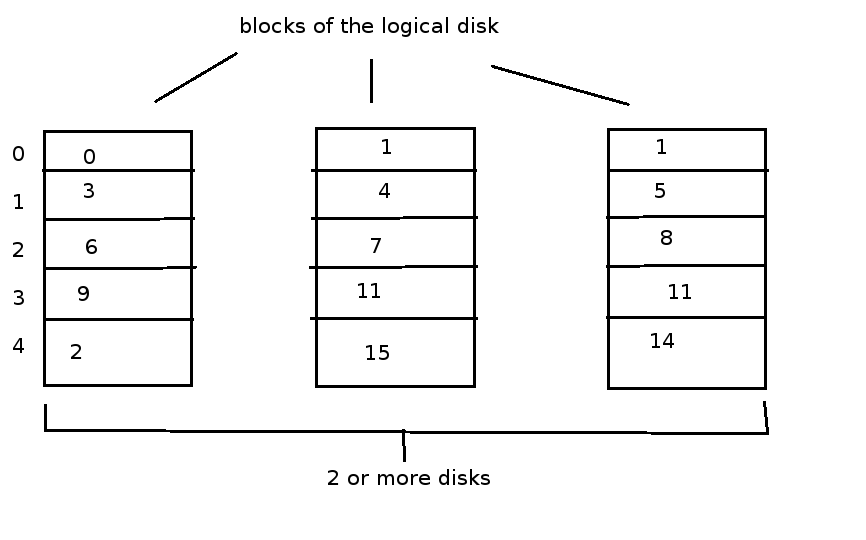
\includegraphics[width=0.8\textwidth]{raid_0.png}
    \caption{}
  \end{center}
\end{figure}

A logical disk in which block n is the block $(n/\#disks)$ of disk $(n \% \#disks)$

Actually the logical disk is divided into chunks which might be larger than the physical block

Also called striping, aims at improving performances.
\begin{figure}[h!]
  \begin{center}
    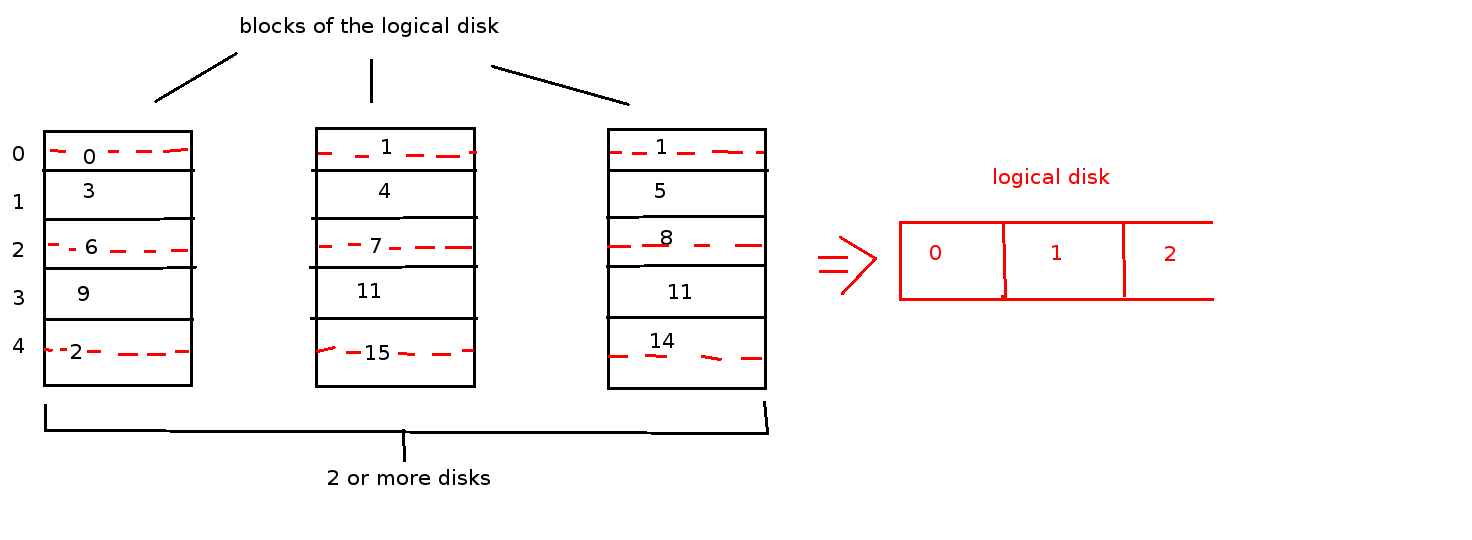
\includegraphics[width=0.8\textwidth]{raid_0_chunks.png}
    \caption{}
  \end{center}
\end{figure}

Advantages:

\begin{itemize}
  \item for large sequential accesses, requests can be issued in parallel on all the disks
  \item some random accesses might be issued in parallel, if they are related to chunks on different disks.
  \item $=>$ Increased Bandwith.
\end{itemize}

Drawbacks:

\begin{itemize}
  \item latency is not improved and might even be degraded
  \item more prone to failure: the probability of failure of the array is larger than the probability of failure of one of the disk
\end{itemize}

\subsection{RAID 1}

Also called mirroring, aims at improving reliability and might improve performances.

\begin{figure}[h!]
  \begin{center}
    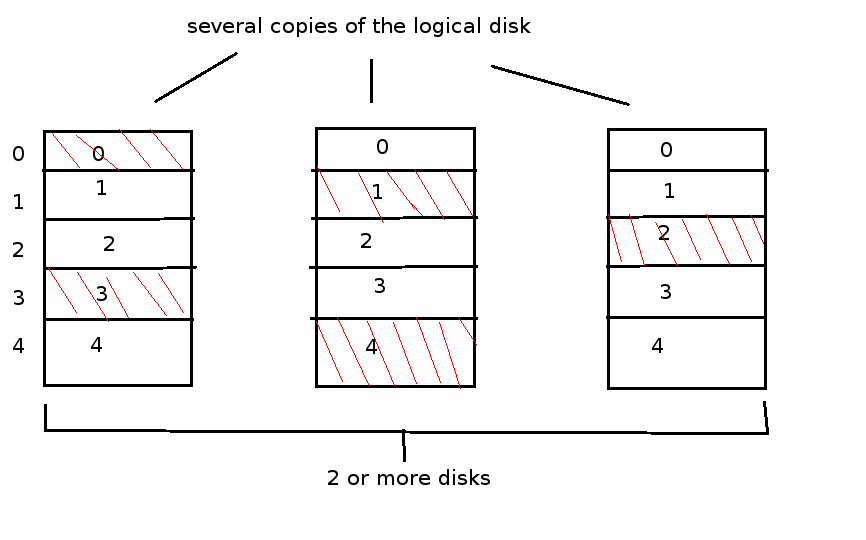
\includegraphics[width=0.8\textwidth]{raid_1.png}
    \caption{}
  \end{center}
\end{figure}

\begin{itemize}
  \item Read accesses can be issued to any of the disks
  \item write accesses are broadcasted in parallel to all the disks
\end{itemize}

Advantages:

\begin{itemize}
  \item performance is improved if read accesses are dispatched on several disks (not always implemented)
  \item can tolerate a number of disks failures of (n-1) (where n is the number of disks)
\end{itemize}

Drawbacks:

\begin{itemize}
  \item n*disks capacity results in a logical disk which has the capacity of a single disk. 
\end{itemize}

\subsection{Hybrid Setups : 0+1, 1+0}
%mettre ça en subfigure,
\begin{figure}[h!]
  \begin{center}
    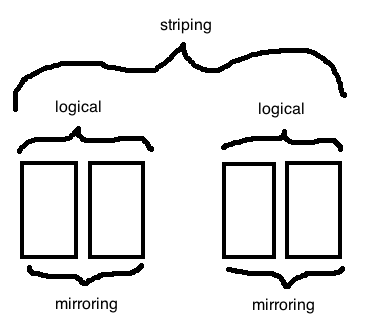
\includegraphics[width=0.4\textwidth]{0_plus_1.png}
    \caption{}
  \end{center}
\end{figure}

Characteristics of the 0+1 setup:
\begin{itemize}
  \item More efficient than a single disk
  \item tolerate 1 failure in the worst case
  \item loss of capacity depends on the number of mirrored disks
\end{itemize}

\begin{figure}[h!]
  \begin{center}
    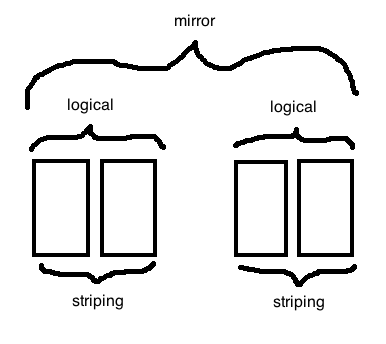
\includegraphics[width=0.4\textwidth]{1_plus_0.png}
    \caption{}
  \end{center}
\end{figure}
Characteristics of the 1+0 setup:
Same as the previous one. 

\subsection{RAID 4}

Combines performance and reliability without loosing too much capacity.

\begin{figure}[h!]
  \begin{center}
    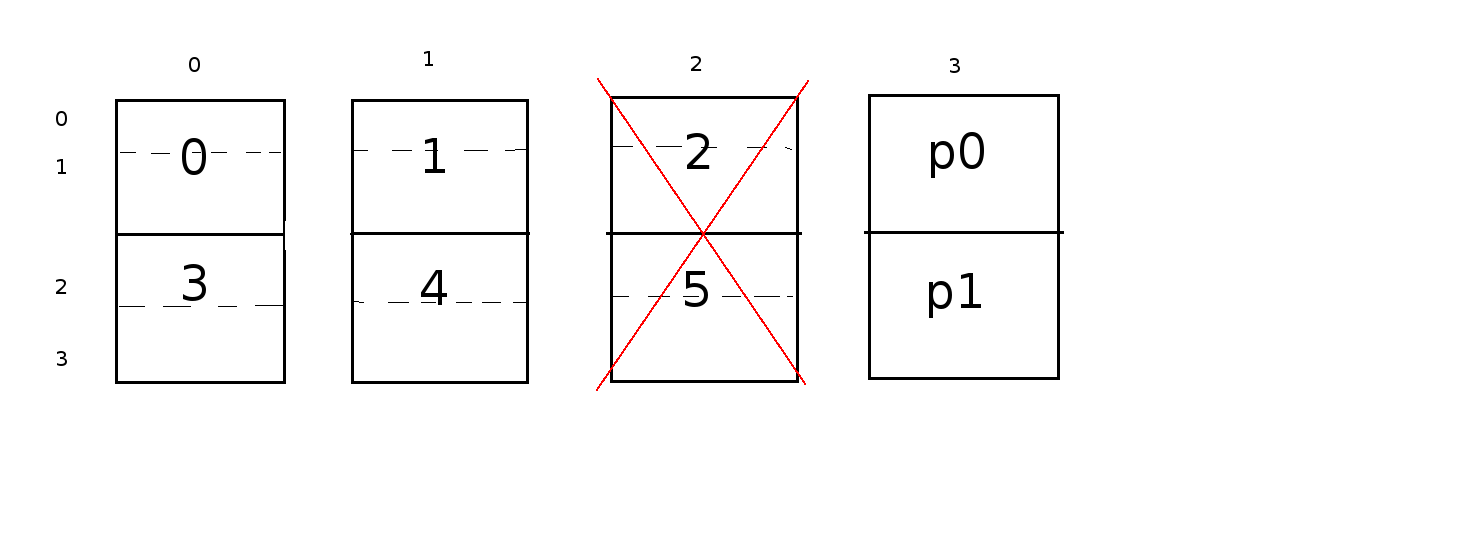
\includegraphics[width=0.8\textwidth]{raid_4.png}
    \caption{}
  \end{center}
\end{figure}

pO contains the parity information computed from chunks 0,1 and 2.
pX contains the parity information computed from chunks X*n, X*n+1, ... , X*n + n-1.

\begin{figure}[h!]
  \begin{center}
    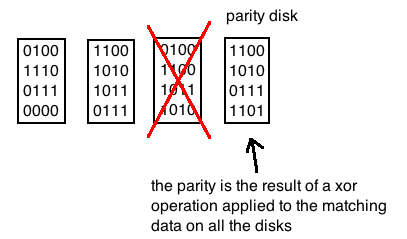
\includegraphics[width=0.8\textwidth]{parity_disk.png}
    \caption{}
  \end{center}
\end{figure}

Advantages :

\begin{itemize}
  \item improved bandwith, similar to a RAID 0 setup with n-1 disks.
  \item tolerates the failure of one disk :
  \begin{itemize}
    \item if this is the parity disk :
    \begin{itemize}
      \item $=>$ no data loss
      \item $=>$ performance remains the same
    \end{itemize}
    \item otherwise :
    \begin{itemize}
      \item lost data can be recomputed : read to all the disk and XOR the results.
      \item large loss of performance.
    \end{itemize}
  \end{itemize}
  \item in the case of a failure, the failing disk has to be replaced and the array rebuild (long operation)
\end{itemize}

Drawbacks :
Small writes : two independant writes to two chunks on different disks cannot be performed in parallel because of the parity disk.

\subsection{RAID 5}

Like RAID 4, except that the parity chunk is stored in a cyclic manner on all the disks.

\begin{figure}[h!]
  \begin{center}
    %\includegraphics[width=0.8\textwidth]{raid_5.png}
    \caption{}
  \end{center}
\end{figure}

\begin{table}[h]
\begin{tabular}{|l|l|l|l|l|l|l|}
\cline{1-1} \cline{3-3} \cline{5-5} \cline{7-7}
$P_0$ &  & 0  &  & 1  &  & 2  \\ \cline{1-1} \cline{3-3} \cline{5-5} \cline{7-7} 
3  &  & $P_1$ &  & 4  &  & 5  \\ \cline{1-1} \cline{3-3} \cline{5-5} \cline{7-7} 
6  &  & 7  &  & $P_2$ &  & 8  \\ \cline{1-1} \cline{3-3} \cline{5-5} \cline{7-7} 
9  &  & 10 &  & 11 &  & $P_3$
\end{tabular}
\end{table}


The parity information for stripe X is stored on disk $(X/n)\%n$.
So for chunk C, it is stored on disk $(X/n(n-1))\%n$.

\begin{figure}[h!]
  \begin{center}
    \includegraphics[width=0.8\textwidth]{parity_disk_raid_5.png}
    \caption{}
  \end{center}
\end{figure}


Advantages :

\begin{itemize}
  \item identical to the ones of RAID 4.
  \item the small writes issue is lessened because some independant write can be issued in parallel.
\end{itemize}

Exemple:

\begin{itemize}
  \item write
      \begin{tabular}{|cccc|}
      \hline
         1&1&0&0 \\
         1&0&0&1 \\
    line
      \end{tabular}
to chunk 1. new parity = old data XOR data XOR old parity.

\item write
      \begin{tabular}{|cccc|}
      \hline
         0&0&0&1 \\
         1&1&1&0 \\
      \hline
      \end{tabular}
to chunk 5. 
\end{itemize}

\subsection{RAID 6}

Additional redundant information to tolerate the failure of two disks (computed from a polynomial in Gallois' Field).

Drawbacks: Computationally intensive, has to be hardware accelerated.

\subsection{Relationship with the OS}

There is a software implementation of levels 0 to 5 in Linux.
Built on top of the device mapper.

\begin{figure}[h!]
  \begin{center}
    \includegraphics[width=0.8\textwidth]{relationship_os.png}
    \caption{}
  \end{center}
\end{figure}

As efficient as hardware solution on a regular desktop machine.
Other implementations are:

\begin{itemize}
  \item fully in hardware (dedicated cards)
  \item partially in hardware (eg parity information computed by the processor with intel chipsets)
\end{itemize}


\end{document}

%%%%%%%%%%%%%%%
%\begin{table}[h]
%\begin{tabular}{|l|l|l|l|l|l|l|}
%\cline{1-1} \cline{3-3} \cline{5-5} \cline{7-7}
%$P_0$ &  & 0  &  & 1  &  & 2  \\ \cline{1-1} \cline{3-3} \cline{5-5} \cline{7-7} 
%3  &  & $P_1$ &  & 4  &  & 5  \\ \cline{1-1} \cline{3-3} \cline{5-5} \cline{7-7} 
%6  &  & 7  &  & $P_2$ &  & 8  \\ \cline{1-1} \cline{3-3} \cline{5-5} \cline{7-7} 
%9  &  & 10 &  & 11 &  & $P_3$
%\end{tabular}
%\end{table}
